\documentclass[a4paper]{scrreprt}

\usepackage[utf8]{inputenc}
\usepackage[T1]{fontenc}
\usepackage[acronym]{glossaries}
\usepackage{graphicx}
\usepackage{booktabs}
\usepackage{pdfpages}
\usepackage{hyperref}
\usepackage{listings}
\usepackage{tablefootnote}
\usepackage{verbatim}
\usepackage{multirow}
\usepackage{subcaption}
\usepackage{floatrow}
\usepackage{siunitx}
\usepackage{wasysym}
\usepackage{natbib}
\usepackage{physics}


\title{Development of an ultra-wide band indoor positioning system}
\author{Antoine Albertelli}
\titlehead{{\Large Ecole Polytechnique Fédérale de Lausanne}\\
    Laboratoire de Systèmes Robotique (LSRO)\\
    Supervisor: Daniel Burnier
}

\begin{document}

\newacronym{imu}{IMU}{Inertial Motion Unit}
\newacronym{dmp}{DMP}{Digital Motion Processor}
\newacronym{uwb}{UWB}{Ultra Wide Band}

\maketitle
\tableofcontents

% TODO: Put each section in its own .tex
\chapter{Introduction}

\section{Requirements}

\section{State of the art}

\begin{enumerate}
    \item Sensor fusion using kalman for 9 axis IMUs is pretty common.
        Usually done using quaternions to represent rotations.
    \item Previous implementations of fusion with UWB focused on a applications of body positioning.
\end{enumerate}

\chapter{Hardware}

\chapter{Positioning algorithm}

\section{Parametric vs non parametric filter}

Parametric filters are filter which take assumptions on the distribution of the state.
The most common assumption is that the distribution is Gaussian.
Non parametric filters, on the other hand, can represent any distribution, and most importantly multi modal ones.

If the problem can be solved using a parametric filter, it is better, as they are computationally less expensive.
Since we are running the code on a small device with little computing power, it is important to take this into account.

\section{First model}

The goal of this model was to create the simplest thing that could possibly work.
It does not account for most issues, but was enough to start work on a simulator for the system.

To simplify the model, the following hypotheses are made:
\begin{enumerate}
    \item The robot moves in the 2D plane, i.e. its pose is described by $\left( x, y, \theta \right)$.
    \item The \gls{imu}'s internal motion processor already outputs $\theta$ (but it drifts).
    \item The \gls{imu} outputs the acceleration vector in body frame $\mathbf{a}^b$.
    \item The inertial frame is aligned with the world frame, i.e. the robot starts with $\theta=0$.
\end{enumerate}

The state contains the position and speed, in world frame:
\begin{equation}
    \mathbf{x} = \begin{pmatrix}x & y & \theta & \dot{x} & \dot{y}\end{pmatrix}^T
\end{equation}

\subsection{Motion model}

The first step is to transform the acceleration from body frame to world frame.

\begin{equation}
    \mathbf{a}^w = R(\theta) \mathbf{a}^b
\end{equation}

The state update equation, using the acceleration as control input

\begin{eqnarray}
    \dv{t} \mathbf{x} &=&
    \begin{pmatrix}
        \dot{x} & 
        \dot{y} &
        0 & % TODO: Maybe take it from acceleration ?
        \mathbf{a}^w_x &
        \mathbf{a}^w_y
    \end{pmatrix}^T \nonumber
    \\&=&
    \begin{pmatrix}
        \dot{x} \\
        \dot{y} \\
        0 \\  % TODO: Maybe take it from acceleration ?
        \cos(\theta) \mathbf{a}^B_x - \sin(\theta) \mathbf{a}^B_y \\
        \sin(\theta) \mathbf{a}^B_x + \cos(\theta) \mathbf{a}^B_y \\
    \end{pmatrix}
\end{eqnarray}

We can turn it into a discrete state update equation using forward Euler:

\begin{equation}
    \mathbf{x}_{t+1} = \mathbf{x}_t + \Delta_t \dv{t} \mathbf{x}
\end{equation}


\subsection{Measurement model}
In this model we have two different measurement functions.
The first one is given by the \gls{dmp} and is directly the heading $\theta$:
\begin{equation}
    h_{DMP}(\mathbf{x}) = \theta
\end{equation}

The second type of measurement is the distance to the UWB anchors.
It is actually a family of functions; each beacon defines a measurement function.
This function is the distance to the position of the beacon, called $\mathbf{b}$.

\begin{equation}
    h_b(\mathbf{x}) = \sqrt{\left(\mathbf{x}_x - \mathbf{b}_x\right)^2 + \left(\mathbf{x}_y - \mathbf{b}_y\right)^2}
\end{equation}

\chapter{Implementation}

\appendix
\chapter{Hardware schematic}
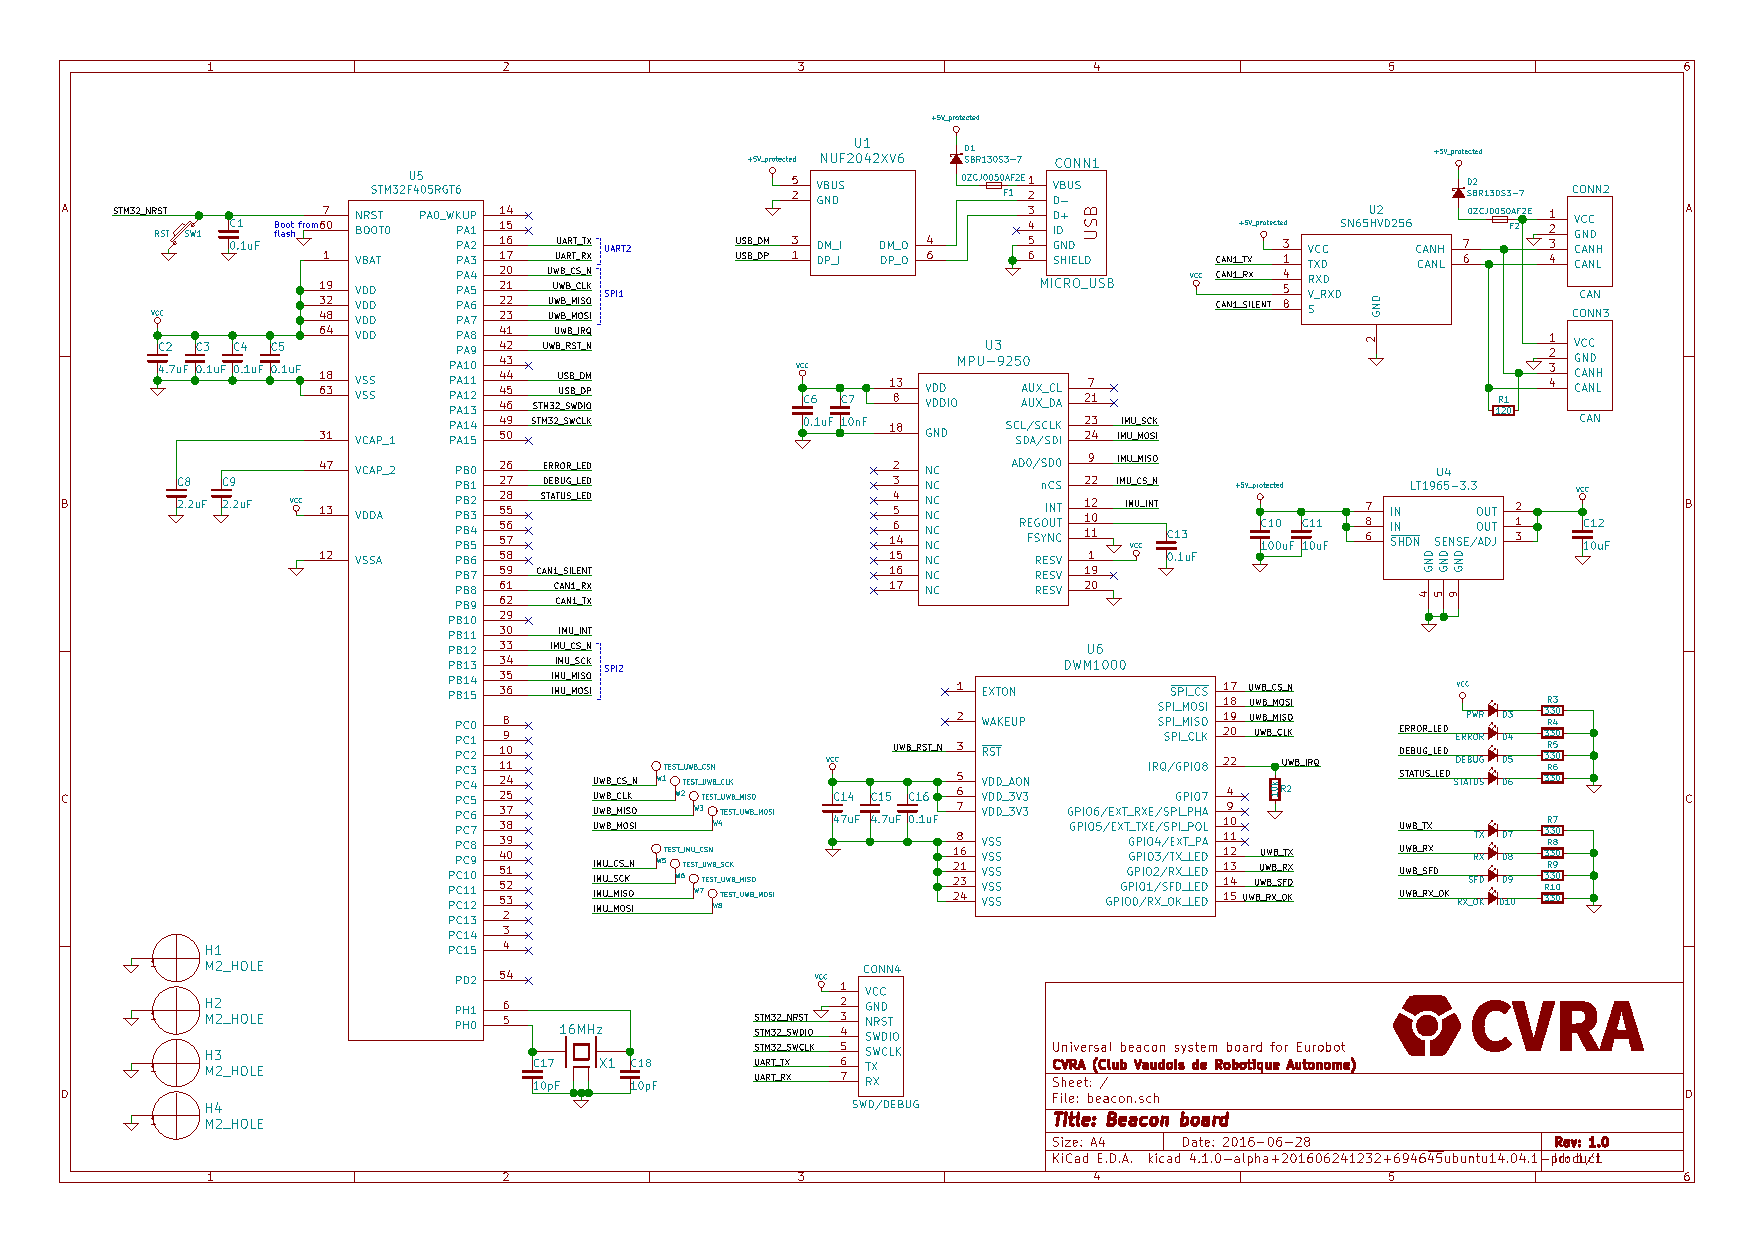
\includepdf[landscape=true]{figures/board_schematic.pdf}


\clearpage
\nocite{*} % tells bibtex to include everything
\bibliographystyle{chicago}
\bibliography{report}

\end{document}
